\documentclass[tikz,border=10pt]{standalone}
\usetikzlibrary{calc}
\begin{document}
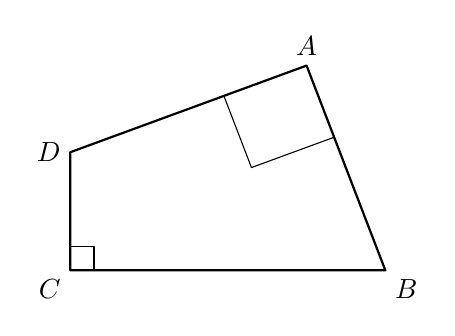
\begin{tikzpicture}[line cap=round,line join=round]
\coordinate (C) at (0,0);
\coordinate (B) at (4,0);
\coordinate (D) at (0,1.5);
\coordinate (A) at (3,2.6);

\draw[thick] (C) -- (B) -- (A) -- (D) -- cycle;

% right angle at C
\draw ($(C)+(0.3,0)$) -- ($(C)+(0.3,0.3)$) -- ($(C)+(0,0.3)$);

% right angle at A aligned with AB and AD
\coordinate (u1) at ($(A)!0.35!(B)$);
\coordinate (u2) at ($(A)!0.35!(D)$);
\draw (u1) -- ($(u1)+(u2)-(A)$) -- (u2);

\node[above] at (A) {$A$};
\node[below right] at (B) {$B$};
\node[below left] at (C) {$C$};
\node[left] at (D) {$D$};
\end{tikzpicture}
\end{document}
